\documentclass[a4paper,12pt]{article}
\usepackage[utf8]{inputenc}
\usepackage[T2A]{fontenc}
\usepackage[russian]{babel}
\usepackage{geometry}
\usepackage{graphicx}
\usepackage{hyperref}
\usepackage{enumitem}
\usepackage{float}
\usepackage{array}
\usepackage{booktabs}
\usepackage{xcolor}


\geometry{left=2.5cm,right=1.5cm,top=2cm,bottom=2cm}

\hypersetup{
	colorlinks=true,
	linkcolor=blue,
	urlcolor=blue
}

\title{\textbf{Проектное предложение}\\ \large{Графопостроитель с автоматической сменой трёх ручек разных цветов   }}
\author{Команда: Орлов М.А. \\ 
	Рудачихин П.А. \\ 
	Свиногонов M.A}
\date{\today}

\begin{document}
	
	\maketitle
	
	\section*{Ментор}
	Преподаватель: \underline{\hspace{5cm}} (ФИО, должность)
	
	\section{Название проекта}
	Графопостроитель с автоматической сменой трёх ручек разных цветов   
	
	\section{Команда}
	\begin{itemize}[leftmargin=*]
		\item \textbf{Орлов М.А.} — ответственный за коммуникацию, электроника и прошивка
		\item \textbf{Рудачихин П.А.} — механика, 3D-моделирование, сборка
		\item \textbf{Свиногонов М.А.} — лазерная резка, пайка, тестирование
	\end{itemize}
	
	\section{Цель проекта}
	Создать настольный плоттер-графопостроитель, обеспечивающий автоматическое воспроизведение векторных изображений на листах бумаги формата A4, с возможностью подъема пишущего узла с помощью сервопривода, сменой трёх ручек разных цветов разных и управлением от персонального компьютера.
	
	\section{Описание функционала}
	Разрабатываемое устройство представляет собой 2D плоттер с неподвижным рабочим столом, над которым перемещается пишущая головка. Основные функциональные возможности и целевые параметры:
	
	\begin{itemize}[leftmargin=*]
		\item \textbf{Рабочее поле:} 210 × 297 мм (формат A4);
		\item \textbf{Механизм подъема ручки:} сервопривод с углом поворота 90°;
		\item \textbf{Автоматическая смена ручек:} сервопривод для захвата на головке + парковочная станция (Tool Changer) на краю стола — смена 3 цветов без вмешательства оператора;
		\item \textbf{Поддерживаемые пишущие инструменты:} ручки;
		\item \textbf{Управление:} USB + Wi-Fi (web-интерфейс);
		\item \textbf{Габариты устройства:} не более 500×400×300 мм;
		\item \textbf{Масса:} не более 5 кг.
	\end{itemize}
	
	\section{Задачи проекта}
	\begin{enumerate}[leftmargin=*]
		\item Провести анализ существующих аналогов и выбрать оптимальную кинематическую схему.
		\item Разработать 3D-модели всех деталей в SolidWorks.
		\item Подготовить файлы для лазерной резки основания из фанеры.
		\item Изготовить детали на 3D-принтере и лазерном резаке.
		\item Выполнить пайку и сборку электронных компонентов.
		\item Собрать механическую часть: валы, подшипники, ременную передачу.
		\item Прошить контроллер и настроить параметры.
		\item Провести калибровку и тестирование.
		\item Подготовить документацию.
	\end{enumerate}
	
	\section{Анализ существующих аналогов}
	
	\subsection*{Roland GS-24}
	Профессиональный графопостроитель. Высокая точность (0,025 мм), промышленная надежность. Недостатки: высокая цена (>100 000 руб.), закрытая архитектура.\\
	\href{https://www.rolanddga.com/products/cutters/gs-24-camm-1-gs-series-desktop-cutter}{Ссылка}
	
	\subsection*{Makeblock XY-Plotter 2.0}
	Наборный плоттер на алюминиевых профилях. Простота сборки, визуальное программирование. Недостатки: ограниченная жесткость, высокая цена (~25 000 руб.).\\
	\href{https://www.makeblock.com/xy-plotter-robot-kit}{Ссылка}
	
	\subsection*{Polargraph (open source)}
	Плоттер с подвесной кареткой на тросах. Простота конструкции, низкая стоимость. Недостатки: сложность калибровки, неравномерность разрешения.\\
	\href{http://www.polargraph.co.uk/}{Ссылка}
	
	\subsection*{CoreXY (DIY 3D принтеры)}
	Кинематика, адаптированная под плоттер. Высокая скорость, компактность. Недостатки: сложность настройки ремней.\\
	\href{https://reprap.org/wiki/CoreXY}{Ссылка}
	
	\subsection*{Сравнительная таблица}
	\begin{table}[H]
		\centering
		\caption{Сравнение аналогов}
		\begin{tabular}{|p{3cm}|p{2.2cm}|p{2.2cm}|p{2.2cm}|p{2.2cm}|}
			\hline
\textbf{Параметр} & \textbf{Roland GS-24} & \textbf{Makeblock} & \textbf{Polargraph} & \textbf{Наш проект} \\
\hline
Стоимость & >100 000 руб. & ~25 000 руб. & <5 000 руб. & <10 000 руб. \\
\hline
Рабочее поле & 584 мм & 300×210 мм & до A2 & A4 \\
\hline
Точность & 0,025 мм & 0,1 мм & 0,3–0,5 мм & $\approx$0,5 мм \\
\hline
Open Source & Нет & Частично & Да & Полностью \\
\hline
Tool Changer & Нет & нет & нет & да \\
\hline
\end{tabular}
\end{table}

\section{Эскиз проекта}
\begin{figure}[H]
	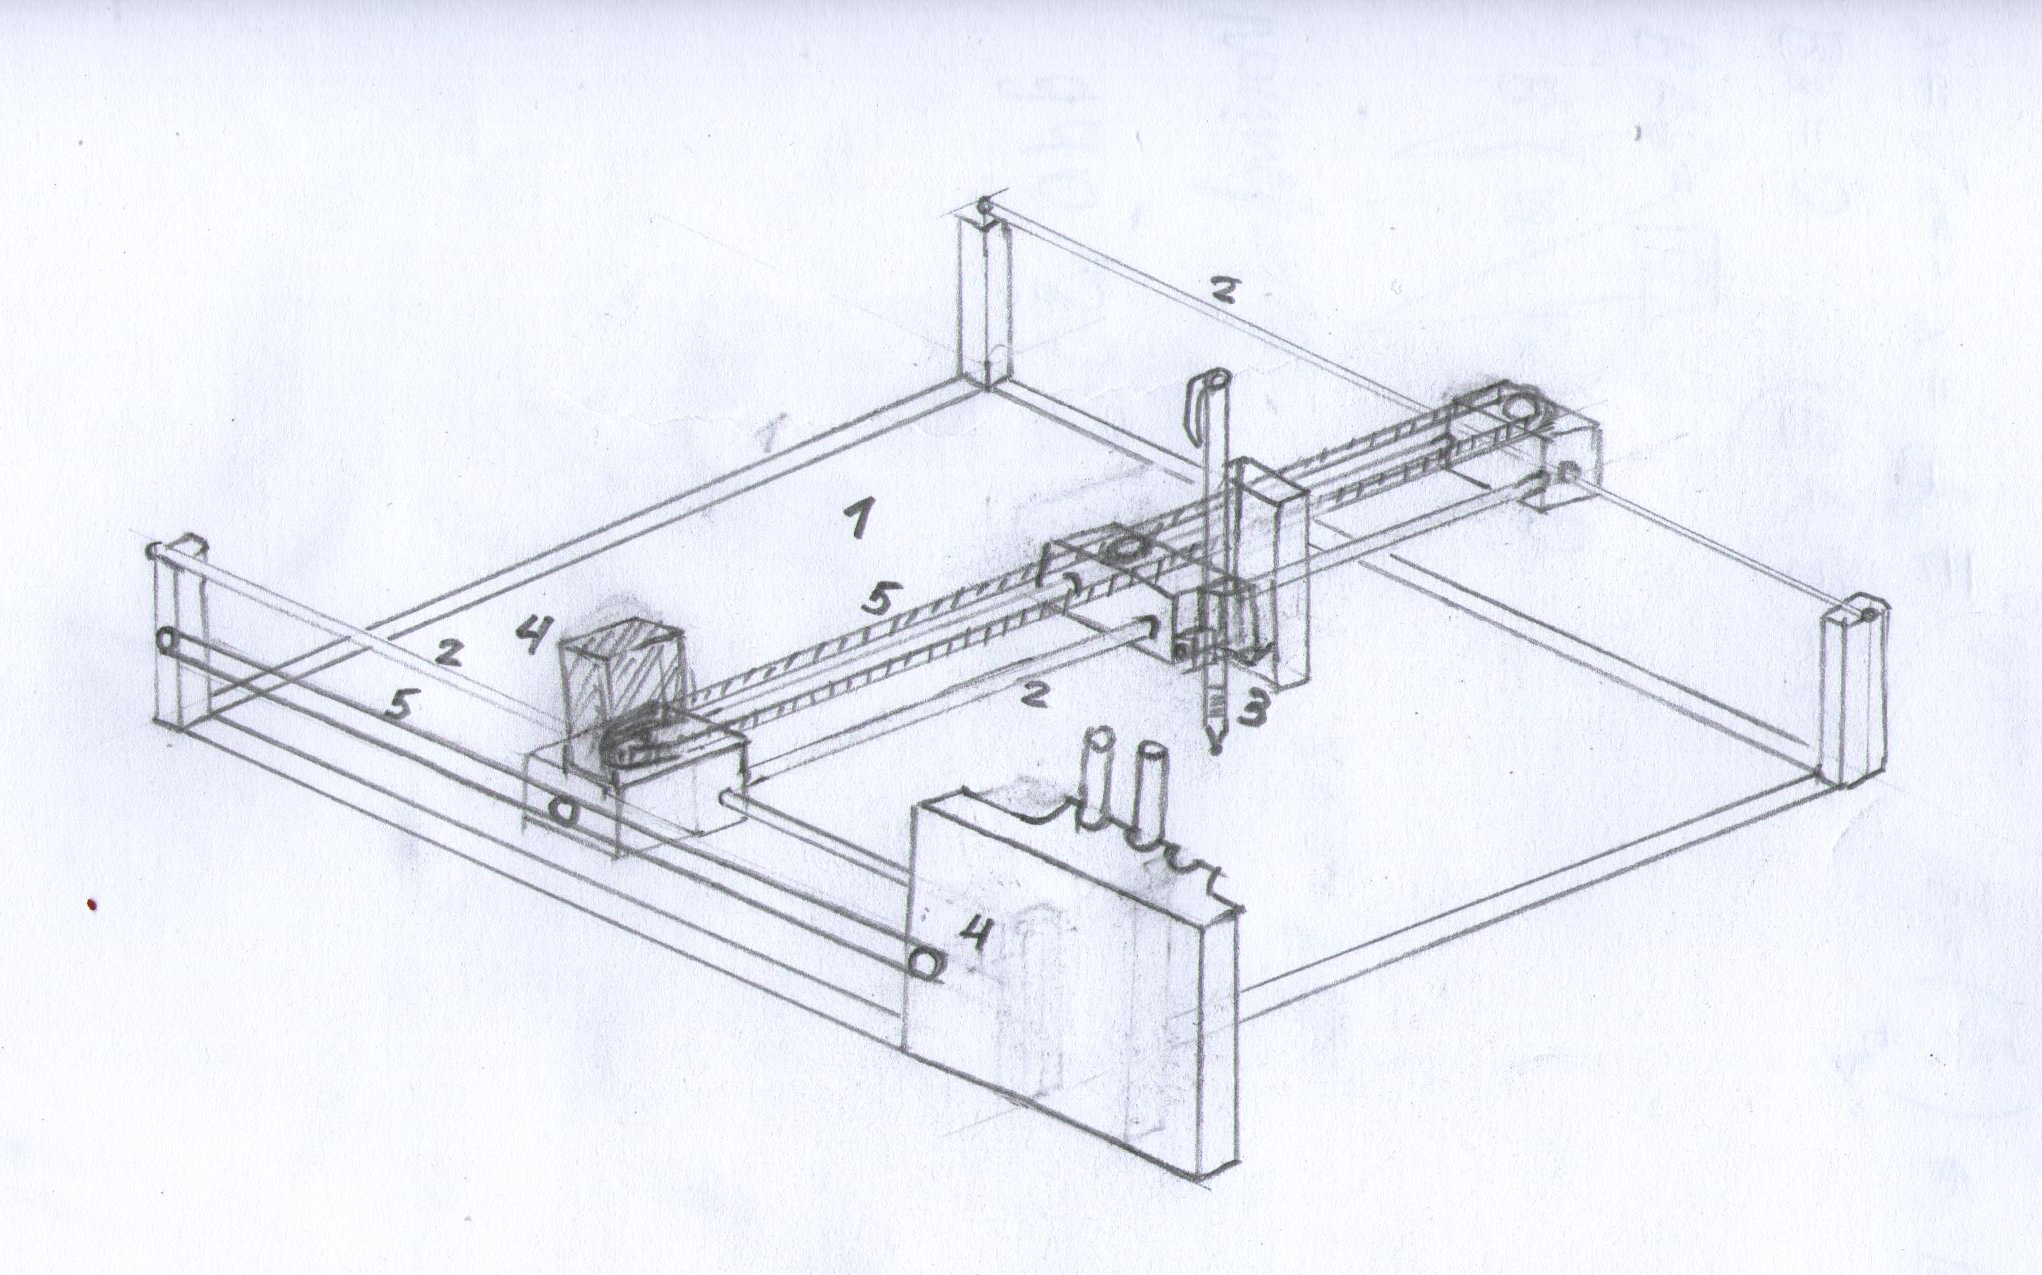
\includegraphics[width=\linewidth]{picture}
\centering
	\caption{Эскиз устройства: 1 — основание,
		2 — валы,
		3 — каретка с сервоприводом,
		4 — шаговые двигатели,
		5 — ремни}
	\label{fig:sketch}
\end{figure}

\section{Элементная база}

\subsection*{Механические компоненты}
\begin{itemize}[leftmargin=*]
\item Валы 400 мм — 2 шт., 350 мм — 2 шт.
\item Линейные подшипники — 8 шт.
\item Алюминиевый профиль — 1,5 м
\item Ремень (6 мм) — 3 м
\item Шкивы (20 зубьев) — 4 шт.
\item Фанера 8 мм — 500×500 мм
\item Крепеж: винты, гайки, подшипники
\end{itemize}

\subsection*{Электронные компоненты}
\begin{itemize}[leftmargin=*]
\item Контроллер: ESP32  или Arduino Mega
\item Драйверы шаговых двигателей, например TMC2208/TMC2209 — 2 шт.
\item Шаговые двигатели — 2 шт.
\item Сервопривод  — 2 шт.
\item Концевые выключатели: 3 шт.
\item Блок питания: 12 В / 5–6 А
\end{itemize}

\subsection*{Расходные материалы}
\begin{itemize}[leftmargin=*]
\item PLA пластик — 500–750 г
\item Припой, флюс, провода, разъемы
\end{itemize}


\end{document}